\documentclass[12pt]{article}
\usepackage[table]{xcolor}
\usepackage[shortlabels]{enumitem}
\usepackage{tabularx,xltabular}
\usepackage{graphicx}
\usepackage{hyperref}
\usepackage{verbatim}
\usepackage{geometry}
\usepackage{ulem}
\usepackage[official]{eurosym}
\usepackage{tikz}
\usetikzlibrary{arrows,backgrounds,calc,decorations.markings,patterns,3d}
\usepackage{pgfplots}
\pgfplotsset{compat = newest}
\usetikzlibrary{fit}
\newcommand\addvmargin[1]{
\usetikzlibrary{arrows}
\node[fit=(current bounding box),inner ysep=#1,inner xsep=0]{};}
\usepackage{cancel}
\usepackage{fontspec}
\usepackage{array}  
\geometry{a4paper, top=2cm, left=2cm, right=2cm, bottom=2cm, headsep=1cm}
\usepackage{tabu}
\usepackage{pst-node}
\usepackage{colortbl}
\usepackage{array}
\usepackage{german}
\setlength\parindent{0pt}
\newcolumntype{?}{!{\vrule width 1pt}}
\usepackage{makecell}
\renewcommand{\arraystretch}{2.5}
\usepackage{pbox}
\usepackage{amssymb}
\usepackage{amsmath}
\usepackage{booktabs}
\newcolumntype{L}[1]{>{\raggedright\let\newline\\\arraybackslash\hspace{0pt}}m{#1}}
\newcolumntype{C}[1]{>{\centering\let\newline\\\arraybackslash\hspace{0pt}}m{#1}}
\newcolumntype{R}[1]{>{\raggedleft\let\newline\\\arraybackslash\hspace{0pt}}m{#1}}
\begin{document}
\rightline{Datum: 08.06.2023}
\centerline{{\Large Tägliche Übungen}} 
\vspace{1cm}
\noindent \\


\begin{xltabular}{\textwidth}{|C{0.75cm}|X|C{0.75cm}|X|}
\arrayrulecolor{black}\hline
a)&$\begin{aligned}
 a=&-7~ \rightarrow ~ 2 \cdot a - 4 \cdot a=?
\end{aligned}$
&
b)&$\begin{aligned}
 a=&12~ \rightarrow ~ 3 \cdot a + 3 \cdot a=?
\end{aligned}$
\\\hline
c)&$\begin{aligned}
 x=&-7~ \rightarrow ~ 3 + x=?
\end{aligned}$
&
d)&$\begin{aligned}
 a=&-10~ \rightarrow ~ 5 - 3 \cdot a=?
\end{aligned}$
\\\hline
e)&$b-43 = 2$
&
f)&$x-25 = 21$
\\\hline
g)&$b+30 = 28$
&
h)&$b+22 = 46$
\\\hline
i)&$y+2 = 9$
&
j)&$a+27 = 11$
\\\hline
k)&$b+42 = 43$
&
l)&$a-25 = 6$
\\\hline
m)&$b-42 = 6$
&
n)&$x+25 = 3$
\\\hline
o)&$b+7 = 34$
&
p)&$a+45 = 48$
\\\hline
q)&$y+22 = 6$
&
r)&$a-41 = 2$
\\\hline
s)&$y+38 = 7$
&
t)&$b+26 = 33$
\\\hline
u)&$a+1 = 31$
&
v)&$b+49 = 31$
\\\hline
w)&$a-44 = 20$
&
x)&$b+31 = 13$
\\\hline
y)&$x+24 = 38$
&
z)&$y+45 = 30$
\\\hline
\end{xltabular}
\vspace{0.5cm}
\newpage
\rightline{Datum: 08.06.2023}
\centerline{{\large Lösungen Tägliche Übungen}} 
\vspace{0.5cm}

\begin{xltabular}{\textwidth}{|C{0.75cm}|X|C{0.75cm}|X|}
\arrayrulecolor{black}\hline
a)&$\begin{aligned}
\textcolor{red}{a=-7} & \rightarrow\\
2 \cdot a - 4 \cdot a=&2 \cdot \textcolor{red}{(-7)} - 4 \cdot \textcolor{red}{(-7)}=14\\
\end{aligned}$
&
b)&$\begin{aligned}
\textcolor{red}{a=12} & \rightarrow\\
3 \cdot a + 3 \cdot a=&3 \cdot \textcolor{red}{12} + 3 \cdot \textcolor{red}{12}=72\\
\end{aligned}$
\\\hline
c)&$\begin{aligned}
\textcolor{red}{x=-7} & \rightarrow\\
3 + x=&3 + \textcolor{red}{(-7)}=-4\\
\end{aligned}$
&
d)&$\begin{aligned}
\textcolor{red}{a=-10} & \rightarrow\\
5 - 3 \cdot a=&5 - 3 \cdot \textcolor{red}{(-10)}=35\\
\end{aligned}$
\\\hline
e)&\begingroup\setlength{\jot}{-0.03cm}
\tikzstyle{background grid}=[draw, black!15,step=.5cm]
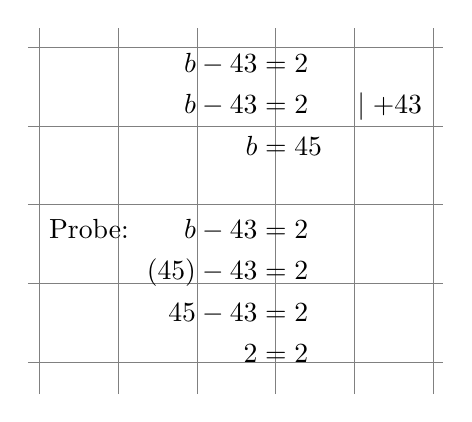
\begin{tikzpicture}[show background grid]
\node[below right] at (0,0.1) {
$\begin{aligned}
b-43  &= 2& &  \\
b - 43 &=2& & \mid + 43\\
b &=45& & 
\\
\\
\mbox{Probe:}\qquad b-43  &= 2& &  \\
\left(45\right)-43  &= 2& &  \\
45-43 &=2& &  \\
2 &=2& &  \\
\end{aligned}$};
\end{tikzpicture}
\endgroup
&
f)&\begingroup\setlength{\jot}{-0.03cm}
\tikzstyle{background grid}=[draw, black!15,step=.5cm]
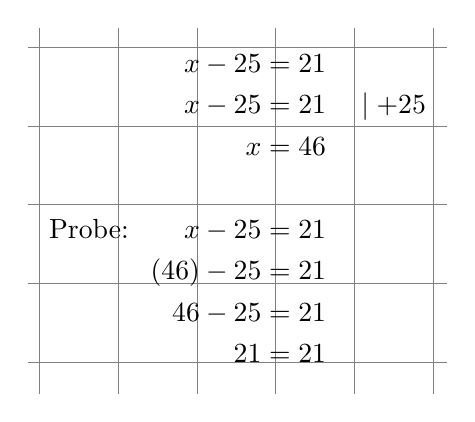
\begin{tikzpicture}[show background grid]
\node[below right] at (0,0.1) {
$\begin{aligned}
x-25  &= 21& &  \\
x - 25 &=21& & \mid + 25\\
x &=46& & 
\\
\\
\mbox{Probe:}\qquad x-25  &= 21& &  \\
\left(46\right)-25  &= 21& &  \\
46-25 &=21& &  \\
21 &=21& &  \\
\end{aligned}$};
\end{tikzpicture}
\endgroup
\\\hline
g)&\begingroup\setlength{\jot}{-0.03cm}
\tikzstyle{background grid}=[draw, black!15,step=.5cm]
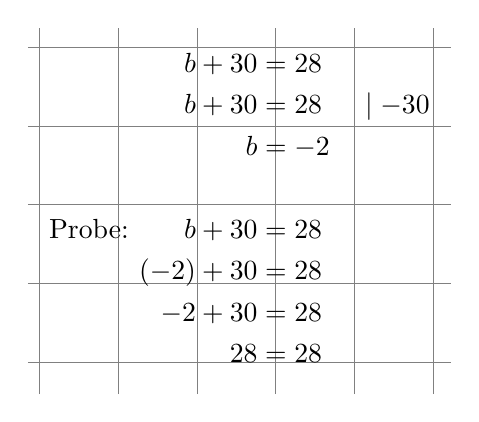
\begin{tikzpicture}[show background grid]
\node[below right] at (0,0.1) {
$\begin{aligned}
b+30  &= 28& &  \\
b + 30 &=28& & \mid - 30\\
b &=-2& & 
\\
\\
\mbox{Probe:}\qquad b+30  &= 28& &  \\
\left(-2\right)+30  &= 28& &  \\
-2+30 &=28& &  \\
28 &=28& &  \\
\end{aligned}$};
\end{tikzpicture}
\endgroup
&
h)&\begingroup\setlength{\jot}{-0.03cm}
\tikzstyle{background grid}=[draw, black!15,step=.5cm]
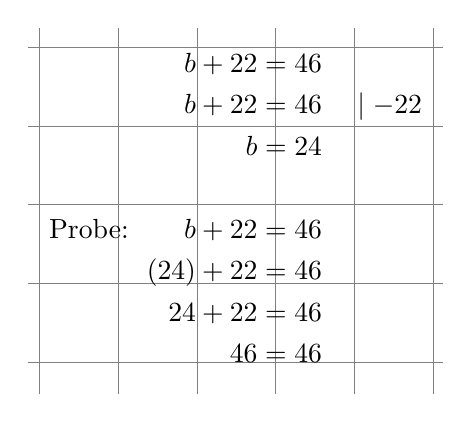
\begin{tikzpicture}[show background grid]
\node[below right] at (0,0.1) {
$\begin{aligned}
b+22  &= 46& &  \\
b + 22 &=46& & \mid - 22\\
b &=24& & 
\\
\\
\mbox{Probe:}\qquad b+22  &= 46& &  \\
\left(24\right)+22  &= 46& &  \\
24+22 &=46& &  \\
46 &=46& &  \\
\end{aligned}$};
\end{tikzpicture}
\endgroup
\\\hline
i)&\begingroup\setlength{\jot}{-0.03cm}
\tikzstyle{background grid}=[draw, black!15,step=.5cm]
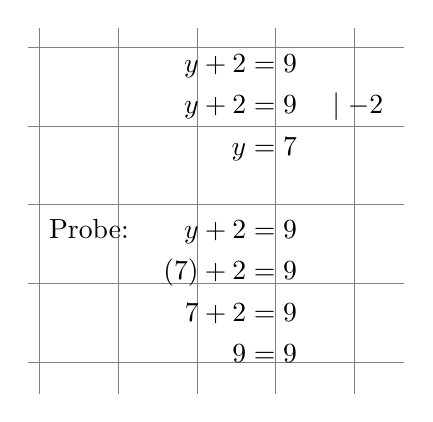
\begin{tikzpicture}[show background grid]
\node[below right] at (0,0.1) {
$\begin{aligned}
y+2  &= 9& &  \\
y + 2 &=9& & \mid - 2\\
y &=7& & 
\\
\\
\mbox{Probe:}\qquad y+2  &= 9& &  \\
\left(7\right)+2  &= 9& &  \\
7+2 &=9& &  \\
9 &=9& &  \\
\end{aligned}$};
\end{tikzpicture}
\endgroup
&
j)&\begingroup\setlength{\jot}{-0.03cm}
\tikzstyle{background grid}=[draw, black!15,step=.5cm]
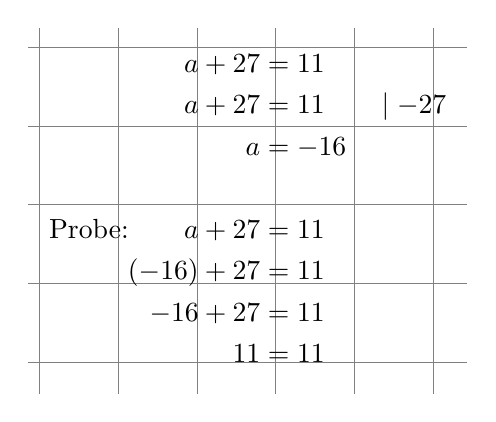
\begin{tikzpicture}[show background grid]
\node[below right] at (0,0.1) {
$\begin{aligned}
a+27  &= 11& &  \\
a + 27 &=11& & \mid - 27\\
a &=-16& & 
\\
\\
\mbox{Probe:}\qquad a+27  &= 11& &  \\
\left(-16\right)+27  &= 11& &  \\
-16+27 &=11& &  \\
11 &=11& &  \\
\end{aligned}$};
\end{tikzpicture}
\endgroup
\\\hline
k)&\begingroup\setlength{\jot}{-0.03cm}
\tikzstyle{background grid}=[draw, black!15,step=.5cm]
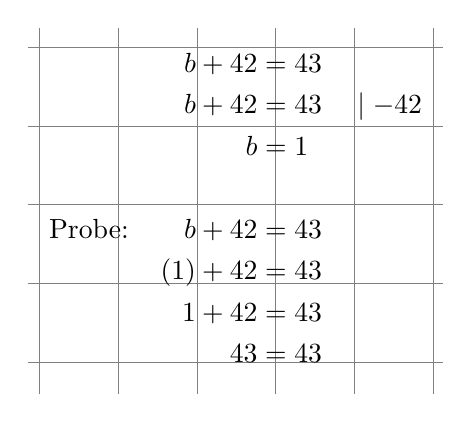
\begin{tikzpicture}[show background grid]
\node[below right] at (0,0.1) {
$\begin{aligned}
b+42  &= 43& &  \\
b + 42 &=43& & \mid - 42\\
b &=1& & 
\\
\\
\mbox{Probe:}\qquad b+42  &= 43& &  \\
\left(1\right)+42  &= 43& &  \\
1+42 &=43& &  \\
43 &=43& &  \\
\end{aligned}$};
\end{tikzpicture}
\endgroup
&
l)&\begingroup\setlength{\jot}{-0.03cm}
\tikzstyle{background grid}=[draw, black!15,step=.5cm]
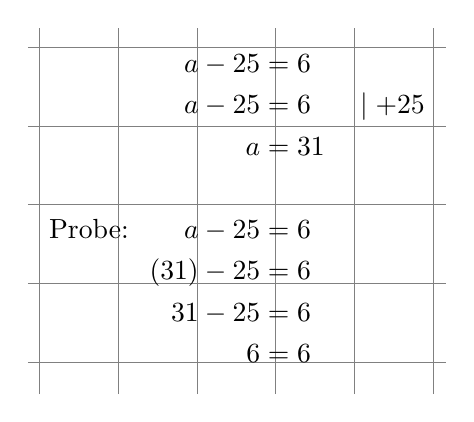
\begin{tikzpicture}[show background grid]
\node[below right] at (0,0.1) {
$\begin{aligned}
a-25  &= 6& &  \\
a - 25 &=6& & \mid + 25\\
a &=31& & 
\\
\\
\mbox{Probe:}\qquad a-25  &= 6& &  \\
\left(31\right)-25  &= 6& &  \\
31-25 &=6& &  \\
6 &=6& &  \\
\end{aligned}$};
\end{tikzpicture}
\endgroup
\\\hline
m)&\begingroup\setlength{\jot}{-0.03cm}
\tikzstyle{background grid}=[draw, black!15,step=.5cm]
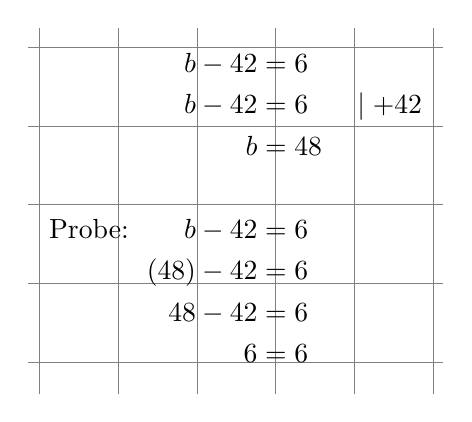
\begin{tikzpicture}[show background grid]
\node[below right] at (0,0.1) {
$\begin{aligned}
b-42  &= 6& &  \\
b - 42 &=6& & \mid + 42\\
b &=48& & 
\\
\\
\mbox{Probe:}\qquad b-42  &= 6& &  \\
\left(48\right)-42  &= 6& &  \\
48-42 &=6& &  \\
6 &=6& &  \\
\end{aligned}$};
\end{tikzpicture}
\endgroup
&
n)&\begingroup\setlength{\jot}{-0.03cm}
\tikzstyle{background grid}=[draw, black!15,step=.5cm]
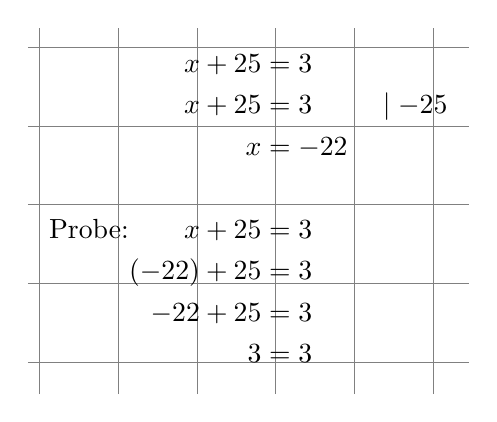
\begin{tikzpicture}[show background grid]
\node[below right] at (0,0.1) {
$\begin{aligned}
x+25  &= 3& &  \\
x + 25 &=3& & \mid - 25\\
x &=-22& & 
\\
\\
\mbox{Probe:}\qquad x+25  &= 3& &  \\
\left(-22\right)+25  &= 3& &  \\
-22+25 &=3& &  \\
3 &=3& &  \\
\end{aligned}$};
\end{tikzpicture}
\endgroup
\\\hline
o)&\begingroup\setlength{\jot}{-0.03cm}
\tikzstyle{background grid}=[draw, black!15,step=.5cm]
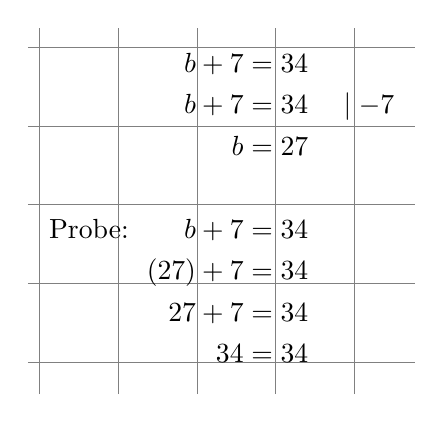
\begin{tikzpicture}[show background grid]
\node[below right] at (0,0.1) {
$\begin{aligned}
b+7  &= 34& &  \\
b + 7 &=34& & \mid - 7\\
b &=27& & 
\\
\\
\mbox{Probe:}\qquad b+7  &= 34& &  \\
\left(27\right)+7  &= 34& &  \\
27+7 &=34& &  \\
34 &=34& &  \\
\end{aligned}$};
\end{tikzpicture}
\endgroup
&
p)&\begingroup\setlength{\jot}{-0.03cm}
\tikzstyle{background grid}=[draw, black!15,step=.5cm]
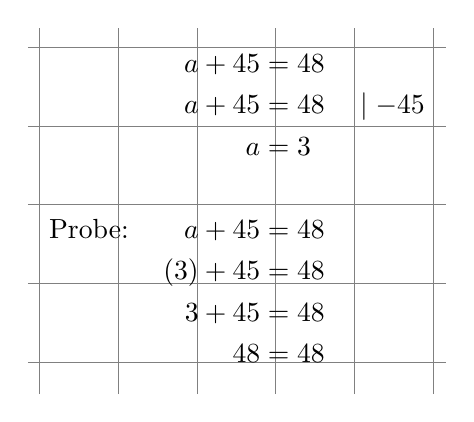
\begin{tikzpicture}[show background grid]
\node[below right] at (0,0.1) {
$\begin{aligned}
a+45  &= 48& &  \\
a + 45 &=48& & \mid - 45\\
a &=3& & 
\\
\\
\mbox{Probe:}\qquad a+45  &= 48& &  \\
\left(3\right)+45  &= 48& &  \\
3+45 &=48& &  \\
48 &=48& &  \\
\end{aligned}$};
\end{tikzpicture}
\endgroup
\\\hline
q)&\begingroup\setlength{\jot}{-0.03cm}
\tikzstyle{background grid}=[draw, black!15,step=.5cm]
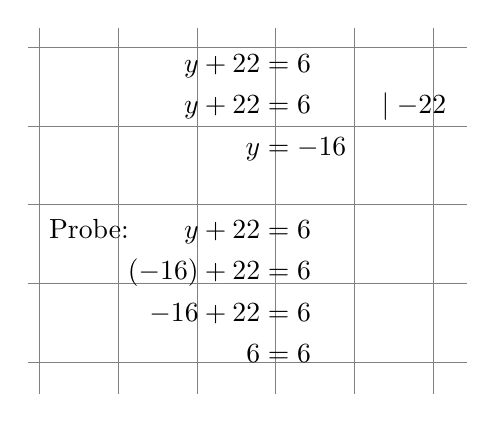
\begin{tikzpicture}[show background grid]
\node[below right] at (0,0.1) {
$\begin{aligned}
y+22  &= 6& &  \\
y + 22 &=6& & \mid - 22\\
y &=-16& & 
\\
\\
\mbox{Probe:}\qquad y+22  &= 6& &  \\
\left(-16\right)+22  &= 6& &  \\
-16+22 &=6& &  \\
6 &=6& &  \\
\end{aligned}$};
\end{tikzpicture}
\endgroup
&
r)&\begingroup\setlength{\jot}{-0.03cm}
\tikzstyle{background grid}=[draw, black!15,step=.5cm]
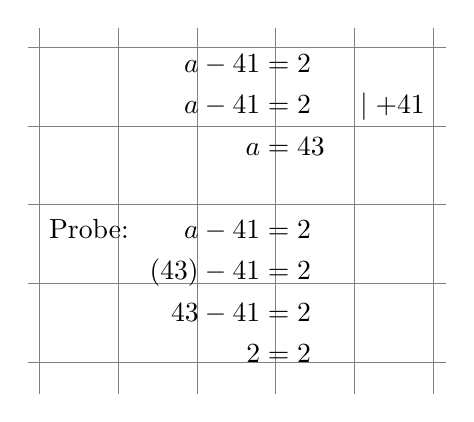
\begin{tikzpicture}[show background grid]
\node[below right] at (0,0.1) {
$\begin{aligned}
a-41  &= 2& &  \\
a - 41 &=2& & \mid + 41\\
a &=43& & 
\\
\\
\mbox{Probe:}\qquad a-41  &= 2& &  \\
\left(43\right)-41  &= 2& &  \\
43-41 &=2& &  \\
2 &=2& &  \\
\end{aligned}$};
\end{tikzpicture}
\endgroup
\\\hline
s)&\begingroup\setlength{\jot}{-0.03cm}
\tikzstyle{background grid}=[draw, black!15,step=.5cm]
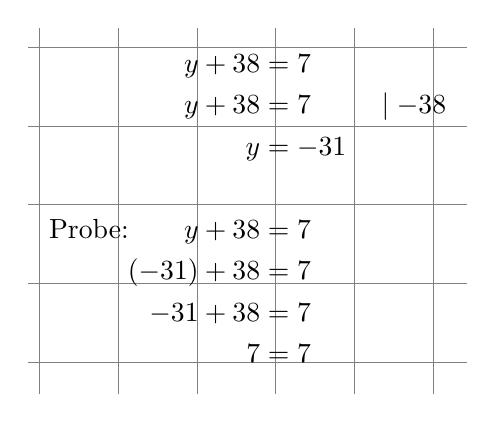
\begin{tikzpicture}[show background grid]
\node[below right] at (0,0.1) {
$\begin{aligned}
y+38  &= 7& &  \\
y + 38 &=7& & \mid - 38\\
y &=-31& & 
\\
\\
\mbox{Probe:}\qquad y+38  &= 7& &  \\
\left(-31\right)+38  &= 7& &  \\
-31+38 &=7& &  \\
7 &=7& &  \\
\end{aligned}$};
\end{tikzpicture}
\endgroup
&
t)&\begingroup\setlength{\jot}{-0.03cm}
\tikzstyle{background grid}=[draw, black!15,step=.5cm]
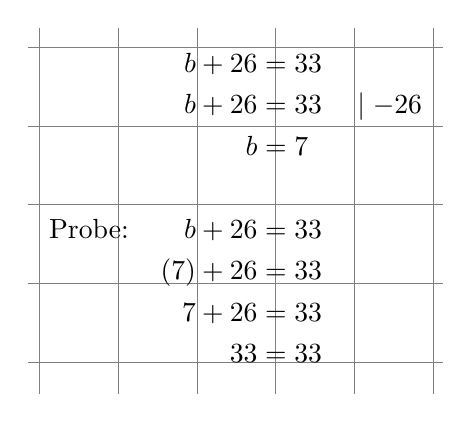
\begin{tikzpicture}[show background grid]
\node[below right] at (0,0.1) {
$\begin{aligned}
b+26  &= 33& &  \\
b + 26 &=33& & \mid - 26\\
b &=7& & 
\\
\\
\mbox{Probe:}\qquad b+26  &= 33& &  \\
\left(7\right)+26  &= 33& &  \\
7+26 &=33& &  \\
33 &=33& &  \\
\end{aligned}$};
\end{tikzpicture}
\endgroup
\\\hline
u)&\begingroup\setlength{\jot}{-0.03cm}
\tikzstyle{background grid}=[draw, black!15,step=.5cm]
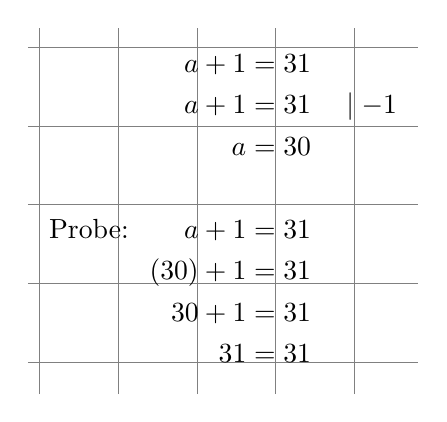
\begin{tikzpicture}[show background grid]
\node[below right] at (0,0.1) {
$\begin{aligned}
a+1  &= 31& &  \\
a + 1 &=31& & \mid - 1\\
a &=30& & 
\\
\\
\mbox{Probe:}\qquad a+1  &= 31& &  \\
\left(30\right)+1  &= 31& &  \\
30+1 &=31& &  \\
31 &=31& &  \\
\end{aligned}$};
\end{tikzpicture}
\endgroup
&
v)&\begingroup\setlength{\jot}{-0.03cm}
\tikzstyle{background grid}=[draw, black!15,step=.5cm]
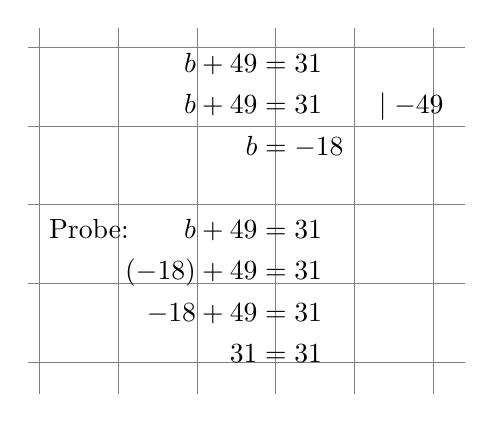
\begin{tikzpicture}[show background grid]
\node[below right] at (0,0.1) {
$\begin{aligned}
b+49  &= 31& &  \\
b + 49 &=31& & \mid - 49\\
b &=-18& & 
\\
\\
\mbox{Probe:}\qquad b+49  &= 31& &  \\
\left(-18\right)+49  &= 31& &  \\
-18+49 &=31& &  \\
31 &=31& &  \\
\end{aligned}$};
\end{tikzpicture}
\endgroup
\\\hline
w)&\begingroup\setlength{\jot}{-0.03cm}
\tikzstyle{background grid}=[draw, black!15,step=.5cm]
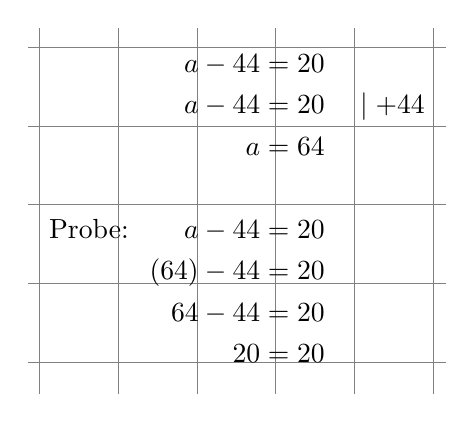
\begin{tikzpicture}[show background grid]
\node[below right] at (0,0.1) {
$\begin{aligned}
a-44  &= 20& &  \\
a - 44 &=20& & \mid + 44\\
a &=64& & 
\\
\\
\mbox{Probe:}\qquad a-44  &= 20& &  \\
\left(64\right)-44  &= 20& &  \\
64-44 &=20& &  \\
20 &=20& &  \\
\end{aligned}$};
\end{tikzpicture}
\endgroup
&
x)&\begingroup\setlength{\jot}{-0.03cm}
\tikzstyle{background grid}=[draw, black!15,step=.5cm]
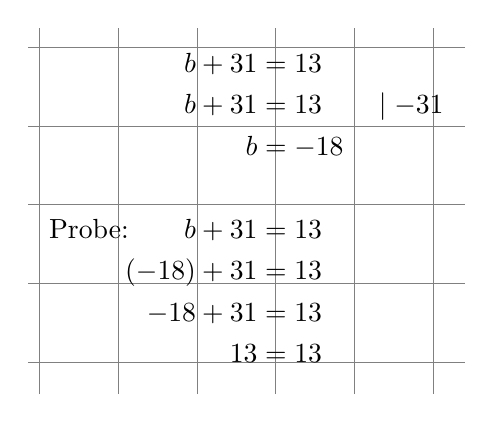
\begin{tikzpicture}[show background grid]
\node[below right] at (0,0.1) {
$\begin{aligned}
b+31  &= 13& &  \\
b + 31 &=13& & \mid - 31\\
b &=-18& & 
\\
\\
\mbox{Probe:}\qquad b+31  &= 13& &  \\
\left(-18\right)+31  &= 13& &  \\
-18+31 &=13& &  \\
13 &=13& &  \\
\end{aligned}$};
\end{tikzpicture}
\endgroup
\\\hline
y)&\begingroup\setlength{\jot}{-0.03cm}
\tikzstyle{background grid}=[draw, black!15,step=.5cm]
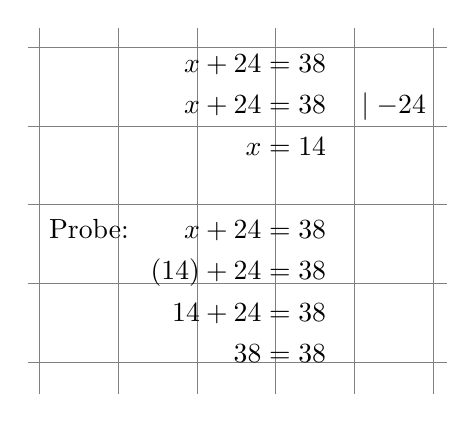
\begin{tikzpicture}[show background grid]
\node[below right] at (0,0.1) {
$\begin{aligned}
x+24  &= 38& &  \\
x + 24 &=38& & \mid - 24\\
x &=14& & 
\\
\\
\mbox{Probe:}\qquad x+24  &= 38& &  \\
\left(14\right)+24  &= 38& &  \\
14+24 &=38& &  \\
38 &=38& &  \\
\end{aligned}$};
\end{tikzpicture}
\endgroup
&
z)&\begingroup\setlength{\jot}{-0.03cm}
\tikzstyle{background grid}=[draw, black!15,step=.5cm]
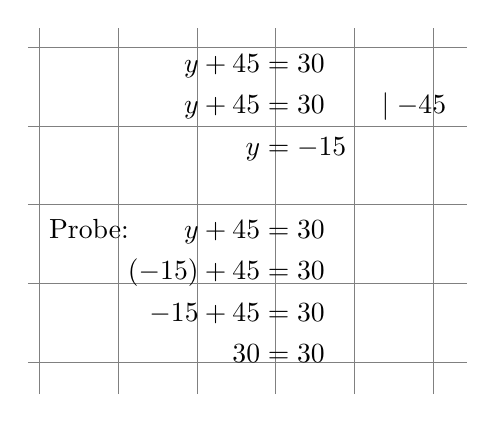
\begin{tikzpicture}[show background grid]
\node[below right] at (0,0.1) {
$\begin{aligned}
y+45  &= 30& &  \\
y + 45 &=30& & \mid - 45\\
y &=-15& & 
\\
\\
\mbox{Probe:}\qquad y+45  &= 30& &  \\
\left(-15\right)+45  &= 30& &  \\
-15+45 &=30& &  \\
30 &=30& &  \\
\end{aligned}$};
\end{tikzpicture}
\endgroup
\\\hline
\end{xltabular}
\vspace{0.5cm}
\end{document}